% Reproduzierbare Vektorquelle für das gleichnamige PDF in Images/.
% Aus dem Repository-Wurzelverzeichnis bauen:
% latexmk -pdf -halt-on-error -interaction=nonstopmode \
%   -outdir=build/figures \
%   Images/sources/algorithm-binary-insertion-sort-search-shift-insert.tex
% cp build/figures/algorithm-binary-insertion-sort-search-shift-insert.pdf Images/
\documentclass[tikz,border=0pt]{standalone}

\usepackage{cmap}
\usepackage[T1]{fontenc}
\usepackage[scaled=0.95]{helvet}
\renewcommand{\familydefault}{\sfdefault}
\usetikzlibrary{arrows.meta}

\definecolor{DiagramNavy}{RGB}{23,54,93}
\definecolor{DiagramGray}{RGB}{127,140,141}
\definecolor{DiagramLightBlue}{RGB}{220,234,247}
\definecolor{DiagramMidBlue}{RGB}{141,185,226}
\definecolor{DiagramOrange}{RGB}{237,125,49}
\definecolor{DiagramPeach}{RGB}{252,228,214}
\definecolor{DiagramGreen}{RGB}{112,173,71}
\definecolor{DiagramLightGreen}{RGB}{217,234,211}
\definecolor{DiagramNearWhite}{RGB}{242,242,242}
\definecolor{DiagramRule}{RGB}{217,226,243}

\begin{document}
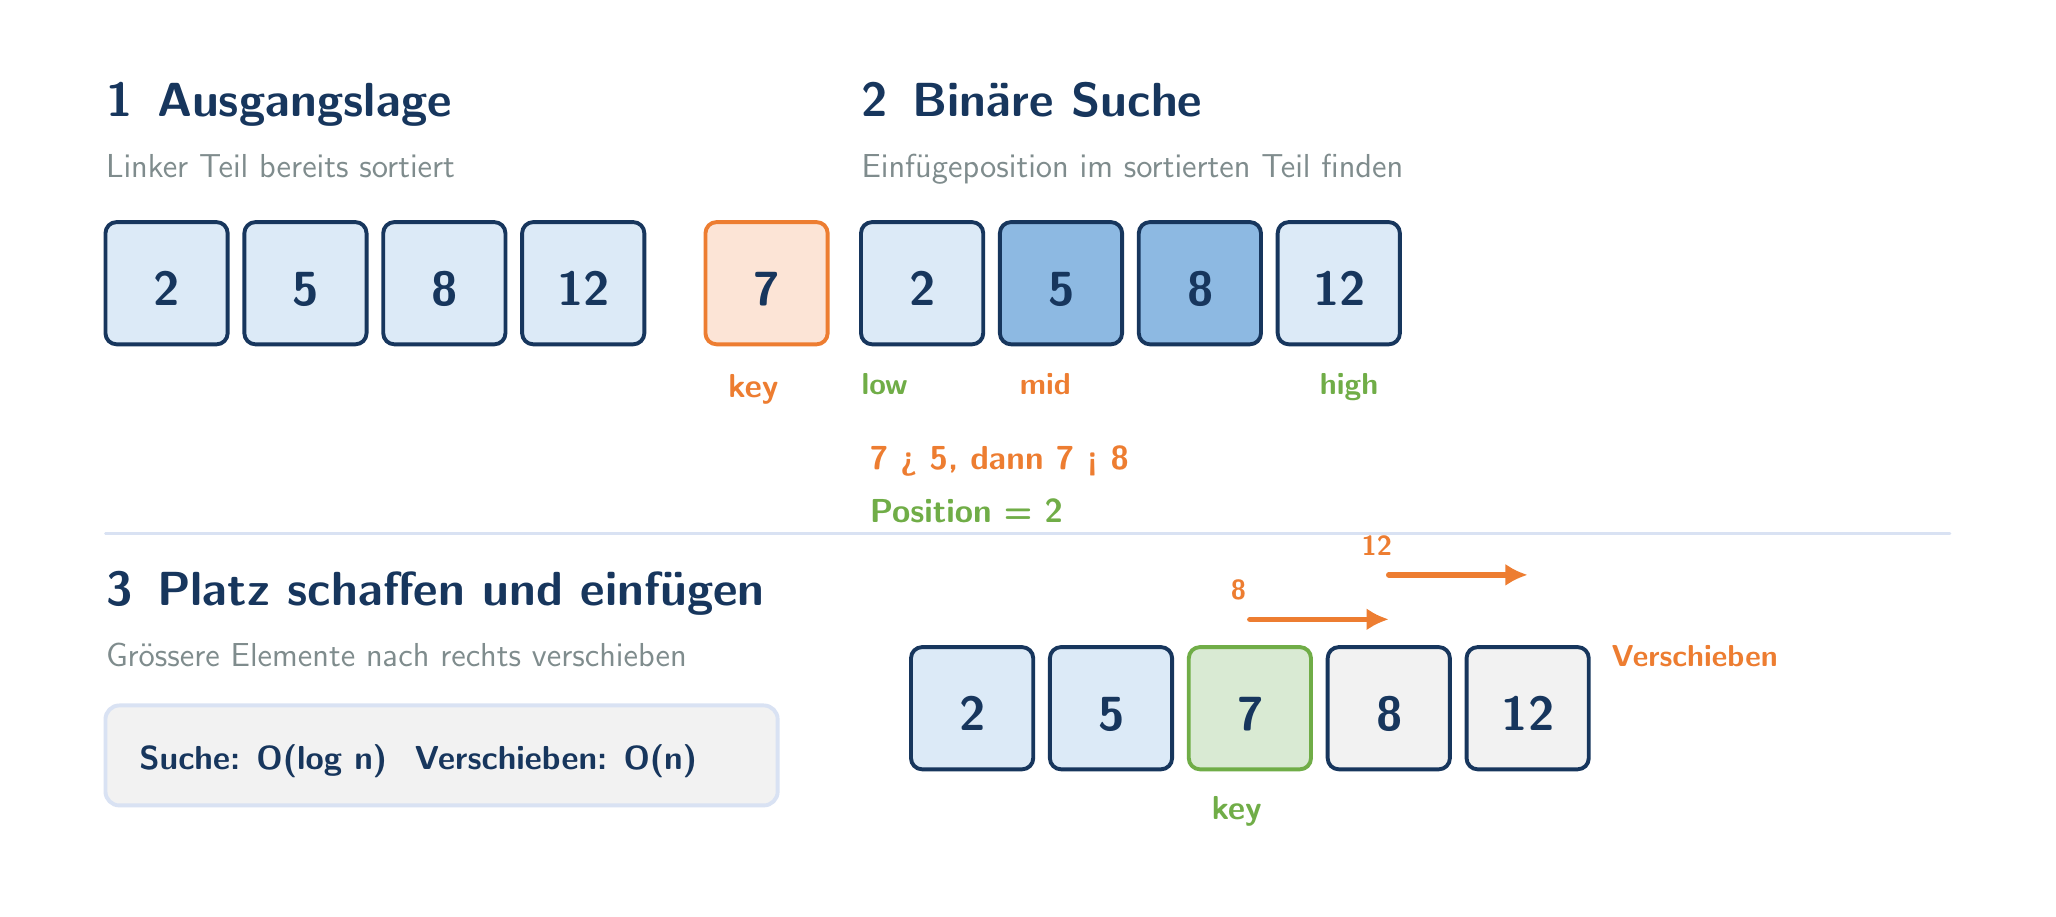
\begin{tikzpicture}[x=1bp,y=1bp,line cap=round,line join=round]
  \path[use as bounding box] (0,0) rectangle (720,310);
  \fill[white] (0,0) rectangle (720,310);

  \tikzset{
    heading/.style={anchor=base west,inner sep=0pt,text=DiagramNavy,
      font=\fontsize{16bp}{16bp}\selectfont\bfseries},
    body/.style={anchor=base west,inner sep=0pt,text=DiagramGray,
      font=\fontsize{12bp}{12bp}\selectfont},
    number/.style={anchor=base west,inner sep=0pt,text=DiagramNavy,
      font=\fontsize{17bp}{17bp}\selectfont\bfseries},
    label/.style={anchor=base west,inner sep=0pt,
      font=\fontsize{11bp}{11bp}\selectfont\bfseries},
    arraybox/.style={rounded corners=4bp,line width=1.4bp,draw=DiagramNavy,
      fill=DiagramLightBlue},
  }

  % 1: Ausgangslage
  \node[heading] at (28,278) {1\hspace{8.9bp}Ausgangslage};
  \node[body] at (28,256) {Linker Teil bereits sortiert};
  \foreach \x/\value in {28/2,78/5,128/8,178/12} {
    \draw[arraybox] (\x,196) rectangle ++(44,44);
    \node[number] at ({\x + (\value == 12 ? 12.55 : 17.27)},210) {\value};
  }
  \draw[rounded corners=4bp,line width=1.4bp,draw=DiagramOrange,fill=DiagramPeach]
    (244,196) rectangle ++(44,44);
  \node[number] at (261.27,210) {7};
  \node[label,text=DiagramOrange,font=\fontsize{12bp}{12bp}\selectfont\bfseries]
    at (252,177) {key};

  % 2: Binäre Suche
  \node[heading] at (300,278) {2\hspace{8.9bp}Binäre Suche};
  \node[body] at (300,256) {Einfügeposition im sortierten Teil finden};
  \draw[arraybox] (300,196) rectangle ++(44,44);
  \draw[arraybox,fill=DiagramMidBlue] (350,196) rectangle ++(44,44);
  \draw[arraybox,fill=DiagramMidBlue] (400,196) rectangle ++(44,44);
  \draw[arraybox] (450,196) rectangle ++(44,44);
  \node[number] at (317.27,210) {2};
  \node[number] at (367.27,210) {5};
  \node[number] at (417.27,210) {8};
  \node[number] at (462.55,210) {12};
  \node[label,text=DiagramGreen] at (300,178) {low};
  \node[label,text=DiagramOrange] at (357,178) {mid};
  \node[label,text=DiagramGreen] at (465,178) {high};
  \node[anchor=base west,inner sep=0pt,text=DiagramOrange,
    font=\fontsize{13bp}{13bp}\selectfont\bfseries]
    at (303,151) {7 > 5, dann 7 < 8};
  \node[anchor=base west,inner sep=0pt,text=DiagramGreen,
    font=\fontsize{13bp}{13bp}\selectfont\bfseries]
    at (303,132) {Position = 2};

  \draw[line width=1bp,DiagramRule] (28,128) -- (692,128);

  % 3: Platz schaffen und einfügen
  \node[heading] at (28,102) {3\hspace{8.9bp}Platz schaffen und einfügen};
  \node[body] at (28,80) {Grössere Elemente nach rechts verschieben};

  \foreach \x/\value in {318/2,368/5} {
    \draw[arraybox] (\x,43) rectangle ++(44,44);
    \node[number] at ({\x + 17.27},57) {\value};
  }
  \draw[rounded corners=4bp,line width=1.4bp,draw=DiagramGreen,fill=DiagramLightGreen]
    (418,43) rectangle ++(44,44);
  \node[number] at (435.27,57) {7};
  \foreach \x/\value/\offset in {468/8/17.27,518/12/12.55} {
    \draw[rounded corners=4bp,line width=1.4bp,draw=DiagramNavy,fill=DiagramNearWhite]
      (\x,43) rectangle ++(44,44);
    \node[number] at ({\x + \offset},57) {\value};
  }
  \node[label,text=DiagramGreen,font=\fontsize{12bp}{12bp}\selectfont\bfseries]
    at (426,25) {key};

  \draw[-{Latex[length=8bp,width=8bp]},line width=2bp,DiagramOrange]
    (440,97) -- (490,97);
  \draw[-{Latex[length=8bp,width=8bp]},line width=2bp,DiagramOrange]
    (490,113) -- (540,113);
  \node[anchor=base west,inner sep=0pt,text=DiagramOrange,
    font=\fontsize{10bp}{10bp}\selectfont\bfseries] at (433,104) {8};
  \node[anchor=base west,inner sep=0pt,text=DiagramOrange,
    font=\fontsize{10bp}{10bp}\selectfont\bfseries] at (480,120) {12};
  \node[label,text=DiagramOrange] at (570,80) {Verschieben};

  \draw[rounded corners=5bp,line width=1.4bp,draw=DiagramRule,fill=DiagramNearWhite]
    (28,30) rectangle (270,66);
  \node[anchor=base west,inner sep=0pt,text=DiagramNavy,
    font=\fontsize{12bp}{12bp}\selectfont\bfseries]
    at (40,43) {Suche: O(log n)\hspace{10bp}Verschieben: O(n)};
\end{tikzpicture}
\end{document}
